%% file: template.tex = LaTeX template for article-like report 
%% init: sometime 1993
%% last: Feb  8 2015  Rob Rutten  Deil
%% site: http://www.staff.science.uu.nl/~rutte101/rrweb/rjr-edu/manuals/student-report/

%% First read ``latex-bibtex-simple-manual.txt'' at
%% http://www.staff.science.uu.nl/~rutte101/Report_recipe.html

%% Start your report production by copying this file into your XXXX.tex.
%% Small changes to the header part will make it an A&A or ApJ manuscript.

%%%%%%%%%%%%%%%%%%%%%%%%%%%%%%%%%%%%%%%%%%%%%%%%%%%%%%%%%%%%%%%%%%%%%%%%%%%%
\documentclass{aa}   %% Astronomy & Astrophysics style class
\usepackage{graphicx,natbib,url,twoopt}
\usepackage[varg]{txfonts}           %% A&A font choice
\usepackage{hyperref}                %% for pdflatex
%%\usepackage[breaklinks]{hyperref}  %% for latex+dvips
%%\usepackage{breakurl}              %% for latex+dvips
\usepackage{pdfcomment}              %% for popup acronym meanings
\usepackage{acronym}                 %% for popup acronym meanings

\hypersetup{
  colorlinks=true,   %% links colored instead of frames
  urlcolor=blue,     %% external hyperlinks
  linkcolor=red,     %% internal latex links (eg Fig)
}

\bibpunct{(}{)}{;}{a}{}{,}    %% natbib cite format used by A&A and ApJ

\pagestyle{plain}   %% undo the fancy A&A pagestyle 

%% Add commands to add a note or link to a reference
\makeatletter
\newcommand{\bibnote}[2]{\@namedef{#1note}{#2}}
\newcommand{\biblink}[2]{\@namedef{#1link}{#2}}
\makeatother

%% Commands to make citations ADS clickers and to add such also to refs
%% May 2014: they give error stops ("Illegal parameter number ..."}
%%   for plain latex with TeX Live 2013; the ad-hoc fixes added below let
%%   latex continue instead of stop within these commands.
%%   Please let me know if you know a better fix!
%%   No such problem when using pdflatex.
\makeatletter
 \newcommandtwoopt{\citeads}[3][][]{%
   \nonstopmode%              %% fix to not stop at error message in latex
   \href{http://adsabs.harvard.edu/abs/#3}%
        {\def\hyper@linkstart##1##2{}%
         \let\hyper@linkend\@empty\citealp[#1][#2]{#3}}%   %% Rutten, 2000
   \biblink{#3}{\href{http://adsabs.harvard.edu/abs/#3}{ADS}}%
   \errorstopmode}            %% fix to resume stopping at error messages 
 \newcommandtwoopt{\citepads}[3][][]{%
   \nonstopmode%              %% fix to not stop at error message in latex
   \href{http://adsabs.harvard.edu/abs/#3}%
        {\def\hyper@linkstart##1##2{}%
         \let\hyper@linkend\@empty\citep[#1][#2]{#3}}%     %% (Rutten 2000)
   \biblink{#3}{\href{http://adsabs.harvard.edu/abs/#3}{ADS}}%
   \errorstopmode}            %% fix to resume stopping at error messages
 \newcommandtwoopt{\citetads}[3][][]{%
   \nonstopmode%              %% fix to not stop at error message in latex
   \href{http://adsabs.harvard.edu/abs/#3}%
        {\def\hyper@linkstart##1##2{}%
         \let\hyper@linkend\@empty\citet[#1][#2]{#3}}%     %% Rutten (2000)
   \biblink{#3}{\href{http://adsabs.harvard.edu/abs/#3}{ADS}}%
   \errorstopmode}            %% fix to resume stopping at error messages 
 \newcommandtwoopt{\citeyearads}[3][][]{%
   \nonstopmode%              %% fix to not stop at error message in latex
   \href{http://adsabs.harvard.edu/abs/#3}%
        {\def\hyper@linkstart##1##2{}%
         \let\hyper@linkend\@empty\citeyear[#1][#2]{#3}}%  %% 2000
   \biblink{#3}{\href{http://adsabs.harvard.edu/abs/#3}{ADS}}%
   \errorstopmode}            %% fix to resume stopping at error messages 
\makeatother

%% Acronyms
\newacro{ADS}{Astrophysics Data System}
\newacro{NLTE}{non-local thermodynamic equilibrium}
\newacro{NASA}{National Aeronautics and Space Administration}

%% Add popups with meaning to acronyms 
%% NB: only show up in Adobe Reader and do not work with \input or \include
\gdef\acp#1{%
  \pdfmarkupcomment[markup=Underline,color={1 1 1},author={{#1}},opacity=0]%
  {{#1}}{{\acl{#1}}}}

%% Spectral species
\def\MgI{\ion{Mg}{I}}          %% A&A; for aastex use \def\MgI{\ion{Mg}{1}} 
\def\MgII{\ion{Mg}{II}}        %% A&A; for aastex use \def\MgII{\ion{Mg}{2}} 

%% Hyphenation
\hyphenation{Schrij-ver}       %% Dutch ij is a single character

%%%%%%%%%%%%%%%%%%%%%%%%%%%%%%%%%%%%%%%%%%%%%%%%%%%%%%%%%%%%%%%%%%%%%%%%%%%%
\begin{document}  

%% simple header.  Change into A&A or ApJ commands for those journals

\twocolumn[{%
\vspace*{4ex}
\begin{center}
  {\Large \bf FYS4150 Project 3: Numerical integration}\\[4ex]
  {\large \bf Peder Forfang, Andreas Ellewsen}\\[4ex]
  %{\large \bf Andreas Ellewsen$^{1}$}\\[4ex]
  %\begin{minipage}[t]{15cm}
  %      $^1$ Institute of theoretical astrophysics\\

%  {\bf Abstract.} We learned how to write nice reports \ldots 

  %\vspace*{2ex}
  %\end{minipage}
\end{center}
}]
%%%%%%%%%%%%%%%%%%%%%%%%%%%%%%%%%%%%%%%%%%%%%%%%%%%%%%%%%%%%%%%%%%%%%%%%%%%%
\section{Introduction}\label{sec:introduction}
%%%%%%%%%%%%%%%%%%%%%%%%%%%%%%%%%%%%%%%%%%%%%%%%%%%%%%%%%%%%%%%%%%%%%%%%%%%%
We are to consider the case of two electrons in a helium atom. The ground state correlation energy between the two electrons can be determined by a six dimensional integral. In this project we will solve such an integral by several different methods: both Gauss-Legendre and Gauss-Laguerre quadrature and Monte Carlo integration, with and without importance sampling.

This is a quantum mechanical problem, and it is not possible to find an analytical solution to Schrödinger's equation for this case. However, we can compute the expectation value of the correlation energy between the two electrons which repell each other via the classical Coulumb interaction. The integral has the form

\begin{equation}
\big \langle \frac{1}{|\bf r_1 - r_2|} \big \rangle = \int_{-\infty}^{\infty}  d{\bf r_1}d{\bf r_2} e^{-2\alpha( r_1 + r_2)} \frac{1}{|\bf r_1 - r_2|}
\end{equation}

The integral can be solved in closed form and has the solution $5\pi^2 / 16^2$.
%%%%%%%%%%%%%%%%%%%%%%%%%%%%%%%%%%%%%%%%%%%%%%%%%%%%%%%%%%%%%%%%%%%%%%%%%%%%
\section{Gauss-Legendre}\label{sec:Gauss-Legendre}
%%%%%%%%%%%%%%%%%%%%%%%%%%%%%%%%%%%%%%%%%%%%%%%%%%%%%%%%%%%%%%%%%%%%%%%%%%%%
First off we will employ the Gauss-Legendre quadrature. Gaussian quadrature differs from other integration methods by the use of orthogonal polynominals, from which we obtain a weight function. In science there are several important orthogonal polynominals which arise from the solution of differential equations. We will use two of these polynominals, the Legendre and the Laguerre, in this project. 

First we start by using the Gauss-Legendre approach. This approach is the general one used if one doesn't see that ones integrand and limits fit well to another polynomial. 

Since our integral goes from $-\infty$ to $+\infty$ for all the variables, and we can't integrate out to those limit we need to define a range over which we integrate. In this case we are lucky, and the integrand goes to zero fairly quickly.
A quick list of calculations shows this:
\begin{equation*}
\begin{aligned}
e^{-1} &\approx 0.37 \\ 
e^{-2} &\approx 0.14 \\
e^{-3} &\approx 0.05 \\
e^{-4} &\approx 0.02 \\
e^{-5} &\approx 0.01 
\end{aligned}
\end{equation*}
So going any further out than $\pm 5$ is probably as waste. Trial and error shows that the results are actually better if we reduce this to $3$ and increase the number of integration points, which makes sense since the contribution is pretty small for $\pm 3$. This can also be seen in figure \ref{exp}.

\begin{figure}
 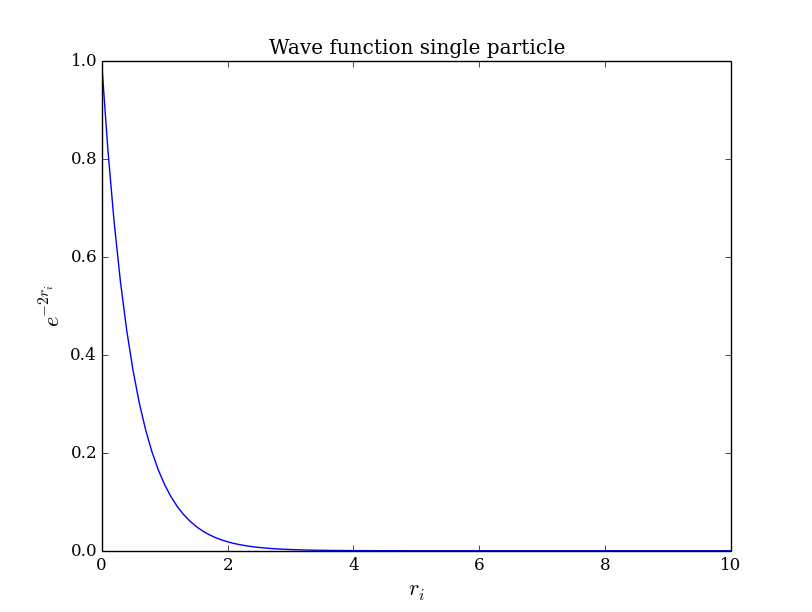
\includegraphics[width=.49\textwidth]{exp.png}
\caption{Wavefunction for single particle. It is clear from the figure that we can approximate the function to be 0 for $r_i > 4$. When doing the calculation we actually see that this can be said for values larger than 3.}
\label{exp}
\end{figure}




Using this method produces a result of $0.194$ with $N = 27$ itegeration points. This takes $t = 28.4$ seconds to calculate. Note that we were unable to get the answer within three leading digits here. This shows that the brute force method may not be the best way to do this. We will explore this in the next section.

%%%%%%%%%%%%%%%%%%%%%%%%%%%%%%%%%%%%%%%%%%%%%%%%%%%%%%%%%%%%%%%%%%%%%%%%%%%%
\section{Gauss-Laguerre}\label{sec:Gauss-Laguerre}
%%%%%%%%%%%%%%%%%%%%%%%%%%%%%%%%%%%%%%%%%%%%%%%%%%%%%%%%%%%%%%%%%%%%%%%%%%%%
Even though using straight forward Gauss-Legendre quadrature does produce a result close to the analystical solution, some thinking can make our result much better. By switching from cartesian to spherical coordinates we can avoid our problem with limits going to infinity. Instead of 6 coordinates going to infinity in both directions, we are left with just the radial parts that go from 0 to infinity. We could try doing the same thing as before in this coordinate system, but there really is no point since our integrand and limits for the radial parts fit so perfectly with the Laguerre polynomials. 

Switching to spherical coordinates changes the integrand to 
\begin{equation}
 I = \int_0^{2\pi}\int_0^{\pi}\int_0^{\infty}r_1^2r_2^2e^{-2\alpha(r_1+r_2)} \frac{sin(\theta_1)sin(\theta_2)}{r_{12}} dr_i d\theta_i d\phi_i
\end{equation}
with 
\begin{equation}
 r_{12} = \sqrt{r_1^2 + r_2^2 -2r_1 r_2cos\beta}
\end{equation}
and
\begin{equation}
 cos(\beta) = cos(\theta_1)cos(\theta_2) + sin(\theta_1)sin(\theta_2)cos(\phi_1 - \phi_2)
\end{equation}
To make this fit with the Laguerre polynomials we need to do a change of variable for the radial parts.
Using the dummy variable $u_i = 2\alpha r_i$, and renaming the variable $r_i$, (which works because the limits for the integral are $0$ and $\infty$) gives
\begin{equation}
\begin{aligned}
&I = \int_0^{2\pi}\int_0^{\pi}\int_0^{\infty}\frac{r_1^2r_2^2e^{-(r_1+r_2)}}{(2\alpha)^5} \frac{sin(\theta_1)sin(\theta_2)}{r_{12}} dr_i d\theta_i d\phi_i
\end{aligned}
\end{equation}

If we use the Laguerre polynomials for the radial parts we absorb $r_i^2 e^{-r_i}$ from each of them.
This means that our integrand becomes 
\begin{equation}
 f(r_1,r_2,\theta_1,\theta_2,\phi_1,\phi_2) =  \frac{sin(\theta_1)\sin(\theta_2)}{(2\alpha)^5 r_{12}},
\end{equation}
where $\phi_1$ and $\phi_2$ are hidden in $r_{12}$.

After several long minutes we arrived at a solution with three leading digits. Using this method produces a result of $0.193$ with $N = 40$ integeration points. This takes $t = 705.4$ seconds to calculate.

%%%%%%%%%%%%%%%%%%%%%%%%%%%%%%%%%%%%%%%%%%%%%%%%%%%%%%%%%%%%%%%%%%%%%%%%%%%%
\section{Monte Carlo}\label{sec:Monte Carlo}
%%%%%%%%%%%%%%%%%%%%%%%%%%%%%%%%%%%%%%%%%%%%%%%%%%%%%%%%%%%%%%%%%%%%%%%%%%%%
We can apply a different method by use of Monte Carlo integration. Monte Carlo makes use of random points in the uniform distribution. The way this works is by a few different things. First we look at our function and decide what distribution best fits the function we want to integrate. In this case it is the exponential distribution but for now we choose to go the brute force way by using the uniform distribution. This is what one does if one does not have a distribution that fits ones function well. When the distribution is chosen one looks at the function in question and finds the hypervolume in which the function produces values larger than zero. In our case we found earlier that we could say that this was in the interval $[-3,3]$. When that is found we multiply our distribution with the length of this volume so that we pick values within the volume which produces values larger than zero for our function. If we now do this N times and then find the average value for the function, we should by multiplying with the size of the distribution we picked values from get the hypervolume under the graph of the function, or in other words, an approximation of the intergral of the function within this volume.

The brute force Monte Carlo method uses much shorter time than the Gaussian quadrature methods.
And we get a result $0.193$ with $N = 200,000,000$ samples. This only takes $29.9$ seconds.
%%%%%%%%%%%%%%%%%%%%%%%%%%%%%%%%%%%%%%%%%%%%%%%%%%%%%%%%%%%%%%%%%%%%%%%%%%%%
\section{Monte Carlo with important sampling}\label{sec:Monte Carlo import}
%%%%%%%%%%%%%%%%%%%%%%%%%%%%%%%%%%%%%%%%%%%%%%%%%%%%%%%%%%%%%%%%%%%%%%%%%%%%
Even though the brute force way produces better results than Gaussian Laguerre quadrature in shorter time we still want to see how close to the right solution we can get. Switching to spherical coordinates, and then using the exponential distribution should give a better result in shorter time. First we make the switch from cartesian to spherical coordinates like we did for Gaussian quadrature. We then note that our function contains and exponential function. Because of this it wise to switch to an exponential distribution for our sampling.

The exponential distribution is
\begin{equation*}
 p(x) = \alpha e^{-\alpha x}
\end{equation*}
which means that
\begin{equation*}
\begin{aligned}
P(x) &= \int_0^x p(x)dx\\
P(x) &= \int_0^x \alpha e^{-\alpha x}dx\\
P(x) &= 1-e^{-\alpha x}\\
e^{-\alpha x} &= 1-P(x)\\
-\alpha x &= ln(1-P(x))\\
x &= -\frac{ln(1-P(x))}{\alpha}\\
\end{aligned}
\end{equation*}
From this it should be clear that if we pick a number P(x) from the uniform distribution, and plug into this equation, we get a number x out in the exponential distribution.
Note that we still use the uniform distribution for the angles $\theta_1$, $\theta_2$, $\phi_1$, and $\phi_2$, multiplying each of them with $\pi$, and $2\pi$ where applicable.
Switching to the exponential distribution means that the exponential in the integral gets absorbed.
This means that our integrand becomes 
\begin{equation}
 f(r_1,r_2,\theta_1,\theta_2,\phi_1,\phi_2) =  \frac{r_1^2 r_2^2}{|\bf r_1 - r_2|} sin(\theta_1)\sin(\theta_2)
\end{equation}
where, as before, $\phi_1$ and $\phi_2$ are hidden in $\bf|r_1 -r_2|$

The Jacobi determinant for this turns out to be the product of all the maxiumum angles $(2\pi)^2\pi^2 = 4\pi^4$. Because that's the volume of the dsitributions we're using for the angles.

Using this method produces a result $ 0.193$ with $N = 750,000$ samples. This takes $t = 0.4$ seconds to calculate. The variance is less than Monte Carlo without importance sampling, which means it is more precise in measuring the positions of the electrons. The time needed to calculate the integral also decreased by a factor of 60, from 30 seconds to half a second.

Since Monte Carlo with importance sampling was so incredibly fast we want to see how close to the right answer we can get within a reasonable time. Running the program with $N = 400,000,000$ results in an answer with five leading digits $0.19276 $, using $t = 179,6 $ seconds. 
%%%%%%%%%%%%%%%%%%%%%%%%%%%%%%%%%%%%%%%%%%%%%%%%%%%%%%%%%%%%%%%%%%%%%%%%%%%%
\section{Conclusions} \label{sec:conclusions}
%%%%%%%%%%%%%%%%%%%%%%%%%%%%%%%%%%%%%%%%%%%%%%%%%%%%%%%%%%%%%%%%%%%%%%%%%%%%
In this project we have seen that Gaussian quadrature can be used to approximate solutions to integrals. We saw that one can do this by either by brute force using Legendre polynomials, or in a more sophisticated way, using Laguerre polynomials (for this case). We also found that the Monte Carlo method produces very good results for the same case. Here we saw that one could use the uniform distribution to make a brute force attempt, giving good results. Or one could use importance sampling by making a mapping over to the exponential distribution, since our integrand contains exponents. By doing this we reduced computation time and improved the result considerably. See table \ref{finalresults} for the details.
\begin{table}
\begin{tabular}{|c|c|c|c|c|}
\hline
Method & Result & Points/Samples & Time & Variance\\
\hline
 Gauss-Legendre & $0.194$ & $27$ & $27.4$s& N/A \\
 \hline
 Gauss-Laguerre & $0.192$ & $30$ & $124.9$s& N/A\\
 \hline
 MC uniform & $0.193$& $200,000,000$ & $29.9$s & 0.00255\\
 \hline
 MC exp & $0.193$& $750000$ & $0.4$s & $0.00121$ \\
 \hline
\end{tabular}
\caption{The results for the different methods, with computation time, number of integration points/samples needed to get the right results with 3 leading digits. Variance is included for MC.}
\label{finalresults}
\end{table}
%%%%%%%%%%%%%%%%%%%%%%%%%%%%%%%%%%%%%%%%%%%%%%%%%%%%%%%%%%%%%%%%%%%%%%%%%%%%
\section{Source code}\label{sec:source}
%%%%%%%%%%%%%%%%%%%%%%%%%%%%%%%%%%%%%%%%%%%%%%%%%%%%%%%%%%%%%%%%%%%%%%%%%%%%
The source code for this document, the c++ project, and the python program for plotting can be found at \url{https://github.com/tellewsen/Project3}.

%%%%%%%%%%%%%%%%%%%%%%%%%%%%%%%%%%%%%%%%%%%%%%%%%%%%%%%%%%%%%%%%%%%%%%%%%%%%
%\begin{acknowledgements}
%\end{acknowledgements}

%%%%%%%%%%%%%%%%%%%%%%%%%%%%%%%%%%%%%%%%%%%%%%%%%%%%%%%%%%%%%%%%%%%%%%%%%%%%
%% references
\section{References}
Computational Physics, Lecture notes Fall 2015, Morten Hjorth-Jensen

%\bibliographystyle{aa-note} %% aa.bst but adding links and notes to references
%\raggedright              %% only for adsaa with dvips, not for pdflatex
%\bibliography{XXX}          %% XXX.bib = your Bibtex entries copied from ADS

\end{document}